% State space diagram of the random intercept cross-lagged panel model (vignette ri-clpm).
\documentclass[tikz, border = 6pt]{standalone}
\usepackage{amsmath}
\usepackage{bm}
\usetikzlibrary{arrows.meta, positioning, calc}
\tikzset{
  lat/.style = {circle, draw, thick, minimum size = 13mm, inner sep = 0pt},
  obs/.style = {rectangle, draw, thick, minimum size = 11mm, inner sep = 1pt},
  noise/.style = {circle, draw, minimum size = 8mm, inner sep = 0pt},
  reg/.style = {-{Stealth[length = 2.5mm]}, thick},
  cov/.style = {{Stealth[length = 2mm]}-{Stealth[length = 2mm]}},
  var/.style = {cov, looseness = 5},
  lab/.style = {font = \footnotesize, fill = white, inner sep = 1pt},
  mat/.style = {font = \small, inner sep = 2pt, align = left},
  dots/.style = {font = \Large}
}
\begin{document}
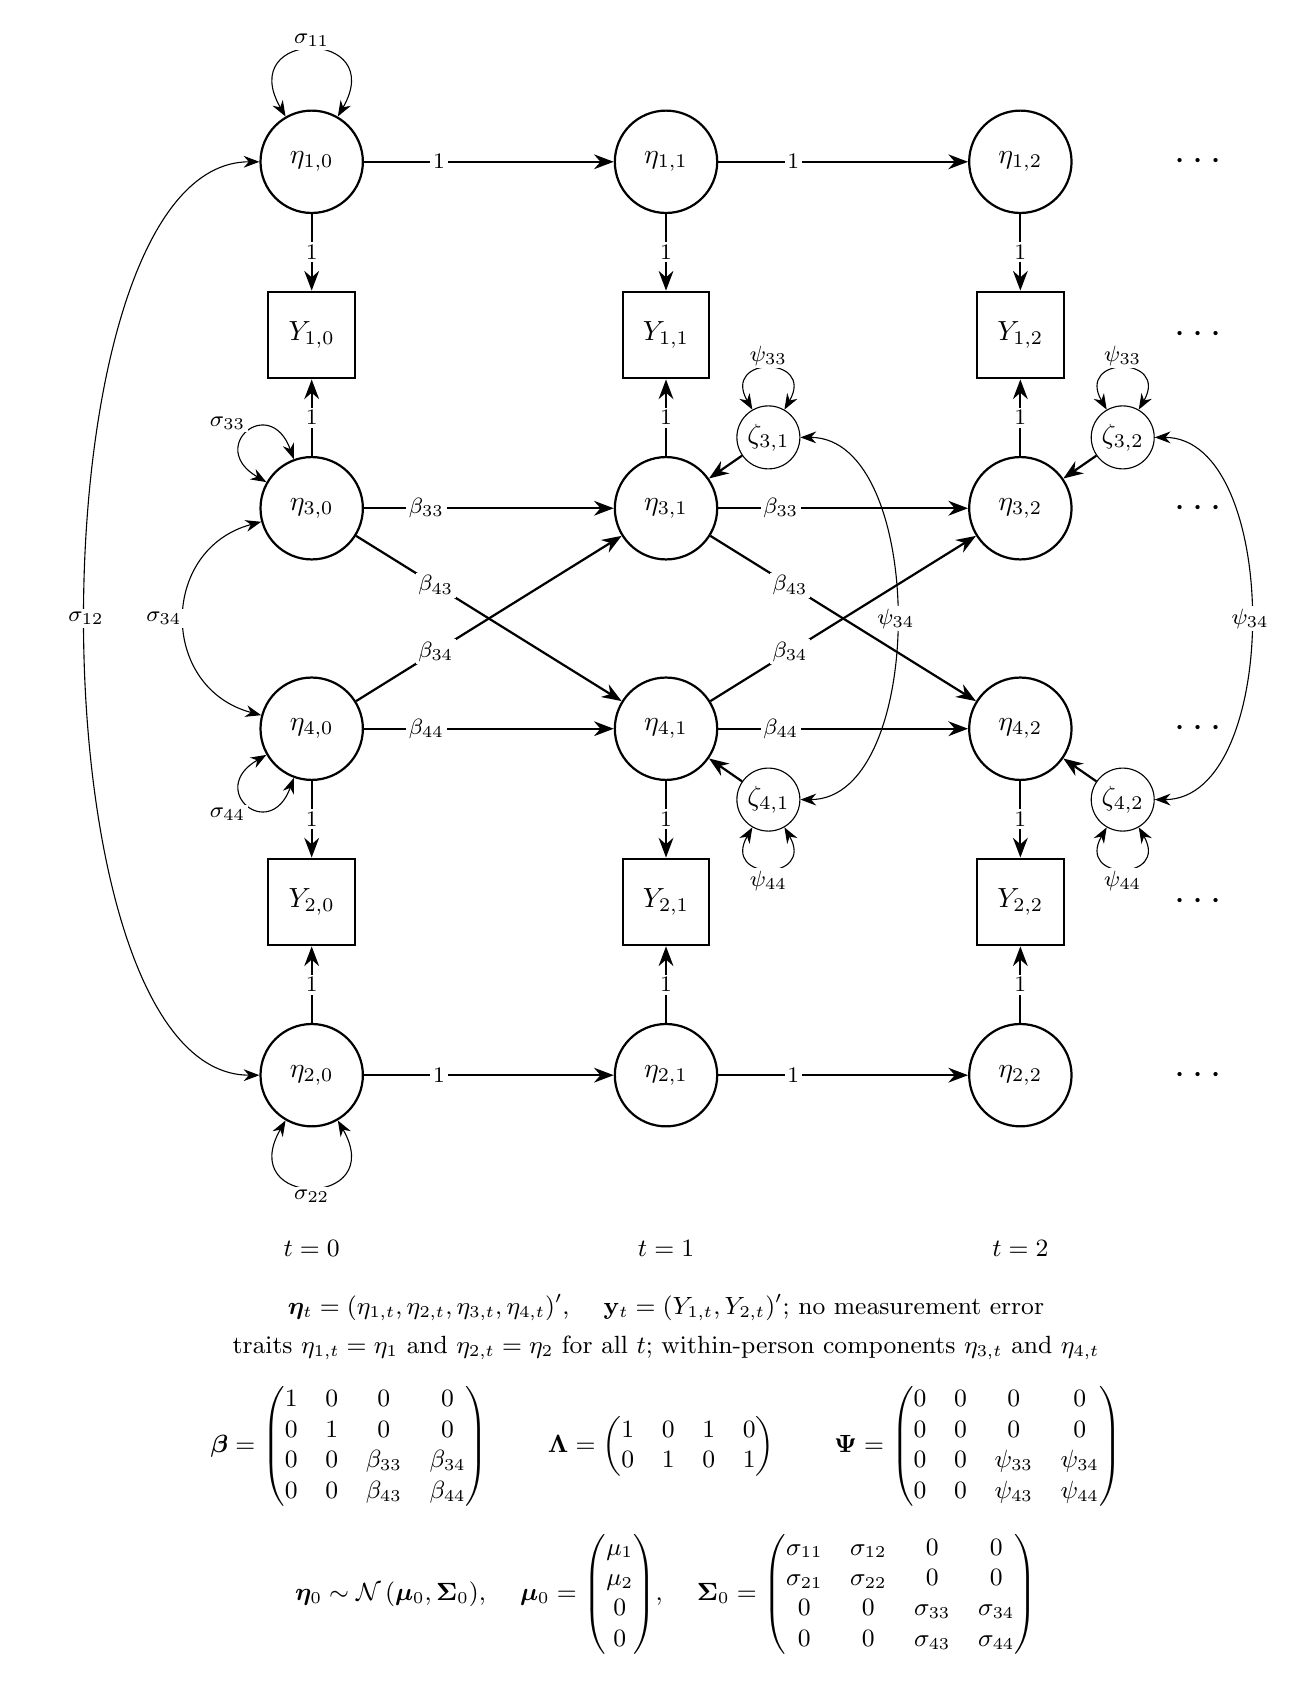
\begin{tikzpicture}
  % occasions
  \foreach \t/\x in {0/0, 1/4.5, 2/9} {
    \node[lat] (a\t) at (\x, 5.4) {$\eta_{1, \t}$};
    \node[obs] (p\t) at (\x, 3.2) {$Y_{1, \t}$};
    \node[lat] (c\t) at (\x, 1.0) {$\eta_{3, \t}$};
    \node[lat] (d\t) at (\x, -1.8) {$\eta_{4, \t}$};
    \node[obs] (q\t) at (\x, -4.0) {$Y_{2, \t}$};
    \node[lat] (b\t) at (\x, -6.2) {$\eta_{2, \t}$};
    \draw[reg] (a\t) -- node[lab] {1} (p\t);
    \draw[reg] (c\t) -- node[lab] {1} (p\t);
    \draw[reg] (d\t) -- node[lab] {1} (q\t);
    \draw[reg] (b\t) -- node[lab] {1} (q\t);
    \node[font = \small] at (\x, -8.4) {$t = \t$};
  }
  % transitions
  \foreach \s/\t in {0/1, 1/2} {
    \draw[reg] (a\s) -- node[lab, pos = 0.3] {1} (a\t);
    \draw[reg] (b\s) -- node[lab, pos = 0.3] {1} (b\t);
    \draw[reg] (c\s) -- node[lab, pos = 0.25] {$\beta_{33}$} (c\t);
    \draw[reg] (d\s) -- node[lab, pos = 0.25] {$\beta_{44}$} (d\t);
    \draw[reg] (d\s) -- node[lab, pos = 0.3] {$\beta_{34}$} (c\t);
    \draw[reg] (c\s) -- node[lab, pos = 0.3] {$\beta_{43}$} (d\t);
  }
  % process noise (within-person components only)
  \foreach \t/\x in {1/4.5, 2/9} {
    \node[noise] (z3\t) at (\x + 1.3, 1.9) {$\zeta_{3, \t}$};
    \node[noise] (z4\t) at (\x + 1.3, -2.7) {$\zeta_{4, \t}$};
    \draw[reg] (z3\t) -- (c\t);
    \draw[reg] (z4\t) -- (d\t);
    \draw[var] (z3\t.60) to[out = 60, in = 120]
      node[lab, above] {$\psi_{33}$} (z3\t.120);
    \draw[var] (z4\t.240) to[out = 240, in = 300]
      node[lab, below] {$\psi_{44}$} (z4\t.300);
    \draw[cov] (z3\t.east) to[out = 0, in = 0, looseness = 0.9]
      node[lab] {$\psi_{34}$} (z4\t.east);
  }
  \foreach \r in {5.4, 3.2, 1.0, -1.8, -4.0, -6.2} {
    \node[dots] at (11.3, \r) {$\cdots$};
  }
  % initial condition
  \draw[var] (a0.60) to[out = 60, in = 120]
    node[lab, above] {$\sigma_{11}$} (a0.120);
  \draw[var] (b0.240) to[out = 240, in = 300]
    node[lab, below] {$\sigma_{22}$} (b0.300);
  \draw[var] (c0.110) to[out = 110, in = 150]
    node[lab, above left] {$\sigma_{33}$} (c0.150);
  \draw[var] (d0.210) to[out = 210, in = 250]
    node[lab, below left] {$\sigma_{44}$} (d0.250);
  \draw[cov] (c0.195) to[out = 195, in = 165, looseness = 1.4]
    node[lab, left] {$\sigma_{34}$} (d0.165);
  \draw[cov] (a0.west) .. controls (-3.6, 5.4) and (-3.6, -6.2) ..
    node[lab] {$\sigma_{12}$} (b0.west);
  % matrices
  \node[mat, align = center, below] at (4.5, -8.9) {%
    $\bm{\eta}_{t} = \left( \eta_{1, t}, \eta_{2, t}, \eta_{3, t},
      \eta_{4, t} \right)^{\prime}$, \quad
    $\mathbf{y}_{t} = \left( Y_{1, t}, Y_{2, t} \right)^{\prime}$;
    no measurement error \\[1mm]
    traits $\eta_{1, t} = \eta_{1}$ and $\eta_{2, t} = \eta_{2}$ for all $t$;
    within-person components $\eta_{3, t}$ and $\eta_{4, t}$ \\[3mm]
    $\bm{\beta} = \begin{pmatrix}
      1 & 0 & 0 & 0 \\ 0 & 1 & 0 & 0 \\
      0 & 0 & \beta_{33} & \beta_{34} \\ 0 & 0 & \beta_{43} & \beta_{44}
    \end{pmatrix}$
    \qquad $\bm{\Lambda} = \begin{pmatrix}
      1 & 0 & 1 & 0 \\ 0 & 1 & 0 & 1
    \end{pmatrix}$
    \qquad $\bm{\Psi} = \begin{pmatrix}
      0 & 0 & 0 & 0 \\ 0 & 0 & 0 & 0 \\
      0 & 0 & \psi_{33} & \psi_{34} \\ 0 & 0 & \psi_{43} & \psi_{44}
    \end{pmatrix}$ \\[3mm]
    $\bm{\eta}_{0} \sim \mathcal{N} \left( \bm{\mu}_{0},
      \bm{\Sigma}_{0} \right)$, \quad
    $\bm{\mu}_{0} = \begin{pmatrix}
      \mu_{1} \\ \mu_{2} \\ 0 \\ 0
    \end{pmatrix}$, \quad
    $\bm{\Sigma}_{0} = \begin{pmatrix}
      \sigma_{11} & \sigma_{12} & 0 & 0 \\
      \sigma_{21} & \sigma_{22} & 0 & 0 \\
      0 & 0 & \sigma_{33} & \sigma_{34} \\
      0 & 0 & \sigma_{43} & \sigma_{44}
    \end{pmatrix}$};
\end{tikzpicture}
\end{document}